%-------------------------
% Resume in Latex
% Author
% License : MIT
%------------------------

%---- Required Packages and Functions ----

\documentclass[a4paper,11pt]{article}
\usepackage{latexsym}
\usepackage{xcolor}
\usepackage{float}
\usepackage{ragged2e}
\usepackage[empty]{fullpage}
\usepackage{wrapfig}
\usepackage{lipsum}
\usepackage{tabularx}
\usepackage{titlesec}
\usepackage{geometry}
\usepackage{marvosym}
\usepackage{verbatim}
\usepackage{enumitem}
\usepackage[hidelinks]{hyperref}
\usepackage{fancyhdr}
\usepackage{multicol}
\usepackage{graphicx}
\usepackage{cfr-lm}
\usepackage[T1]{fontenc}
\setlength{\multicolsep}{0pt} 
\pagestyle{fancy}
\fancyhf{} % clear all header and footer fields
\fancyfoot{}
\renewcommand{\headrulewidth}{0pt}
\renewcommand{\footrulewidth}{0pt}
\geometry{left=1.4cm, top=0.8cm, right=1.2cm, bottom=1cm}
% Adjust margins
%\addtolength{\oddsidemargin}{-0.5in}
%\addtolength{\evensidemargin}{-0.5in}
%\addtolength{\textwidth}{1in}
\usepackage[most]{tcolorbox}
\tcbset{
	frame code={}
	center title,
	left=0pt,
	right=0pt,
	top=0pt,
	bottom=0pt,
	colback=gray!20,
	colframe=white,
	width=\dimexpr\textwidth\relax,
	enlarge left by=-2mm,
	boxsep=4pt,
	arc=0pt,outer arc=0pt,
}

\urlstyle{same}

\raggedright
\setlength{\tabcolsep}{0in}

% Sections formatting
\titleformat{\section}{
  \vspace{-4pt}\scshape\raggedright\large
}{}{0em}{}[\color{black}\titlerule \vspace{-7pt}]

%-------------------------
% Custom commands
\newcommand{\resumeItem}[2]{
  \item{
    \textbf{#1}{\hspace{0.5mm}#2 \vspace{-0.5mm}}
  }
}

\newcommand{\resumePOR}[3]{
\vspace{0.5mm}\item
    \begin{tabular*}{0.97\textwidth}[t]{l@{\extracolsep{\fill}}r}
        \textbf{#1}\hspace{0.3mm}#2 & \textit{\small{#3}} 
    \end{tabular*}
    \vspace{-2mm}
}

\newcommand{\resumeSubheading}[4]{
\vspace{0.5mm}\item
    \begin{tabular*}{0.98\textwidth}[t]{l@{\extracolsep{\fill}}r}
        \textbf{#1} & \textit{\footnotesize{#4}} \\
        \textit{\footnotesize{#3}} &  \footnotesize{#2}\\
    \end{tabular*}
    \vspace{-2.4mm}
}

\newcommand{\resumeProject}[4]{
\vspace{0.5mm}\item
    \begin{tabular*}{0.98\textwidth}[t]{l@{\extracolsep{\fill}}r}
        \textbf{#1} & \textit{\footnotesize{#3}} \\
        \footnotesize{\textit{#2}} & \footnotesize{#4}
    \end{tabular*}
    \vspace{-2.4mm}
}

\newcommand{\resumeSubItem}[2]{\resumeItem{#1}{#2}\vspace{-4pt}}

% \renewcommand{\labelitemii}{$\circ$}
\renewcommand{\labelitemi}{$\vcenter{\hbox{\tiny$\bullet$}}$}

\newcommand{\resumeSubHeadingListStart}{\begin{itemize}[leftmargin=*,labelsep=0mm]}
\newcommand{\resumeHeadingSkillStart}{\begin{itemize}[leftmargin=*,itemsep=1.7mm, rightmargin=2ex]}
\newcommand{\resumeItemListStart}{\begin{justify}\begin{itemize}[leftmargin=3ex, rightmargin=2ex, noitemsep,labelsep=1.2mm,itemsep=0mm]\small}

\newcommand{\resumeSubHeadingListEnd}{\end{itemize}\vspace{2mm}}
\newcommand{\resumeHeadingSkillEnd}{\end{itemize}\vspace{-2mm}}
\newcommand{\resumeItemListEnd}{\end{itemize}\end{justify}\vspace{-2mm}}
\newcommand{\cvsection}[1]{%
\vspace{2mm}
\begin{tcolorbox}
    \textbf{\large #1}
\end{tcolorbox}
    \vspace{-4mm}
}

\newcolumntype{L}{>{\raggedright\arraybackslash}X}%
\newcolumntype{R}{>{\raggedleft\arraybackslash}X}%
\newcolumntype{C}{>{\centering\arraybackslash}X}%
%---- End of Packages and Functions ------

%-------------------------------------------
%%%%%%  CV STARTS HERE  %%%%%%%%%%%
%%%%%% DEFINE ELEMENTS HERE %%%%%%%
\newcommand{\name}{Fanisus R} % Your Name
\newcommand{\course}{Bachelor of Technology} % Your Course
\newcommand{\phone}{6382468758} % Your Phone Number
\newcommand{\emailb}{fanisusr@karunya.edu.in} %Email
\newcommand{\github}{Ferrb9579} %Github
\newcommand{\website}{https://612151820.xyz/} %Website
\newcommand{\linkedin}{fanisus} %linkedin



\begin{document}
\fontfamily{cmr}\selectfont
%----------HEADING-----------------
\parbox{2.35cm}{%

    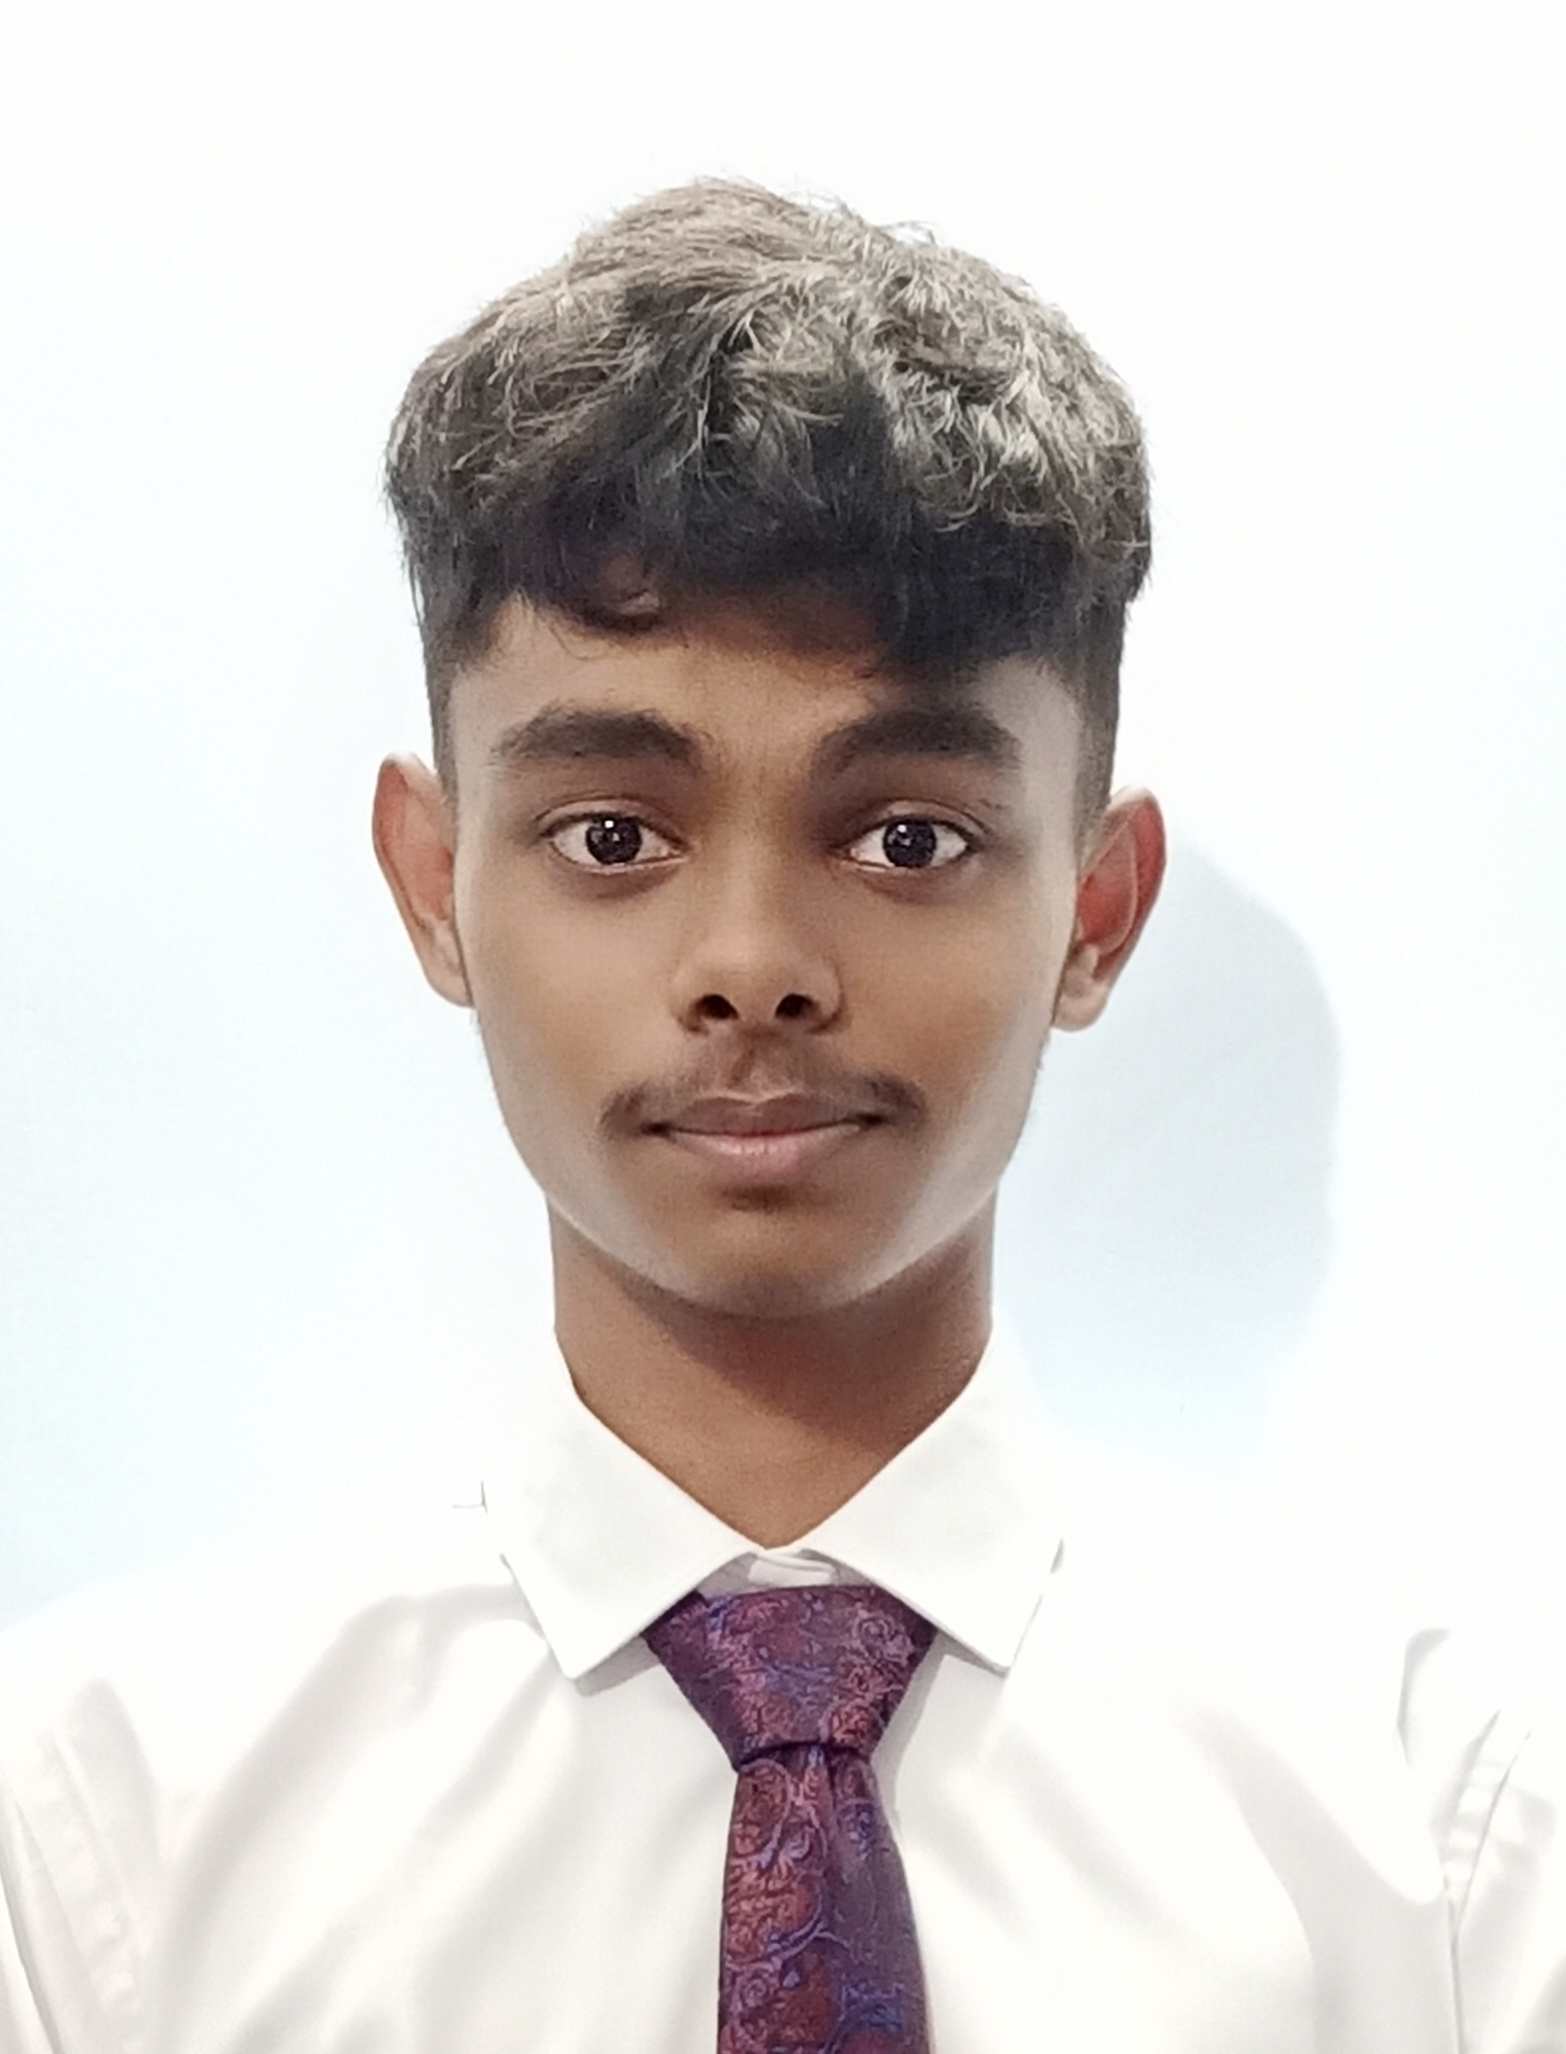
\includegraphics[width=2cm,clip]{Fanisus.jpg}

}\parbox{\dimexpr\linewidth-2.8cm\relax}{
    \begin{tabularx}{\linewidth}{L r}
        \textbf{\LARGE \name}                                      & +91-\phone                                                               \\

        \course                                                    & \href{mailto:\emailb}{\emailb}                                           \\
        {Computer Science and Engineering}                         & \href{https://github.com/\github}{Github} $|$ \href{\website}{Website}   \\
        {Karunya Institute of Technology and Sciences, Coimbatore} & \href{https://www.linkedin.com/in/\linkedin/}{linkedin.com/in/\linkedin}
    \end{tabularx}
}



%-----------EDUCATION-----------------

\section{Education}
\setlength{\tabcolsep}{5pt} % Default value: 6pt
% \renewcommand{\arraystretch}{1.1} % Default value: 1https://www.overleaf.com/project/61fc166d7eab8975b2ab74d0
\small{\begin{tabularx}
        {\dimexpr\textwidth-3mm\relax}{|c|C|c|c|}
        \hline
        \textbf{Degree/Certificate } & \textbf{Institute/Board}                                 & \textbf{CGPA/Percentage} & \textbf{Year} \\
        \hline
        B.Tech. (CSE)                & Karunya Institute of Technology and Sciences, Coimbatore & 8.43                     & 2023-2027     \\ %Optional
        \hline
        Senior Secondary             & CBSE Board                                               & 76.8\%                   & 2023          \\
        \hline
        Secondary                    & CBSE Board                                               & 78.4\%                   & 2021          \\
        \hline
    \end{tabularx}}
\vspace{-2mm}

%-----------EXPERIENCE-----------------
\section{Experience}
\resumeSubHeadingListStart

\resumeSubheading
{ProPlusLogics}{Coimbatore}
{Flutter Intern}{Mar 2023 - Apr. 2023}
\resumeItemListStart
\item {Developed key user interface components in Flutter for a Doctor Appointment mobile application, focusing on intuitive design and user experience.}
\item {Designed and implemented the user registration and appointment scheduling screens for a Doctor Appointment app using Flutter, adhering to project specifications and deadlines.}
\resumeItemListEnd

% \resumeSubheading
%   {Personal Life.}{Bengaluru, India}
%   {Full Stack Developer Intern}{Dec. 2018 - Jan. 2019}
%   \resumeItemListStart
% \item {Developed web app using ReactJS and deployed the app to AWS EC2 using Docker.}
%     \item {Made website mobile-friendly and increased Google web dev score by 50 points.}
% \resumeItemListEnd

\resumeSubHeadingListEnd
\vspace{-5.5mm}
%-----------PROJECTS-----------------
\section{Projects}
\resumeSubHeadingListStart

\resumeProject
{Maxxel } %Project Name
{NodeJS} %Project Name, Location Name
{Dec. 2021 - Jan. 2022} %Event Dates
{\href{https://what-to-watch-next.herokuapp.com/}{Live Url}
|  {\href{https://github.com/ankit0696/what-to-watch-next}{Github}} } %Website
\resumeItemListStart
\item {Developed a Discord music bot with moderation features,
            music playback, and queue management using discord.js}
\resumeItemListEnd

\resumeProject
  {Battle Turtle} %Project Name
  {ReactJS, TailwindCSS, NodeJS, ExpressJS} %Project Name, Location Name
  {Feb. 2025 - Apr. 2025} %Event Dates

  \resumeItemListStart
    \item {Developed a online competitive coding platform, where students can solve problems and get graded}
\resumeItemListEnd

% \resumeProject
%   {Kisa Mitra(SIH 2019) } %Project Name
%   {Web Portal for Ministry of Agriculture to view the predicted crop yield data in geo-refrenced map. } %Project Name, Location Name
%   {Feb. 2019 - Mar. 2019} %Event Dates
%   {\href{https://github.com/ankit0696/kisan_mitra}{Github}} %Website
%   \resumeItemListStart
%      \item {\textbf{Tools \& technologies used}: QGIS, Java, HTML, CSS, JS, ChartistJS}
%     \item {Created APIs to fetch crop production data and displayed them into Geo-refrenced Map.}
% \resumeItemListEnd


\resumeSubHeadingListEnd
\vspace{-5.5mm}


\section{Technical Skills}
\resumeHeadingSkillStart
\resumeSubItem{Programming: } % Category
{JavaScript, Flutter/Dart, Rust, Python, SQL}
\resumeSubItem{Tools \& OS: } % Category
{Docker, Git, Linux, Windows, VS Code } % Skills
\resumeSubItem{Libraries/Frameworks: } % Category
{ExpressJS, PrismaJS}

\resumeSubItem{Web Skills: } % Category
{ReactJS, Flutter}
%  \resumeSubItem{Operating Systems}
%  {Windows, Linux*} 
% \hfill \textit{\footnotesize{* Elementary proficiency}} \hspace{3mm}
\resumeHeadingSkillEnd


\section{Positions of Responsibility}
\vspace{-0.4mm}
\resumeSubHeadingListStart
% \resumePOR{Co-Head,} % Position
%     {K-Hacks Web and App Dev, KITS} %Club,Event
%     {Present} %Tenure Period
\resumePOR{Coordinator, } % Position
{K-Hacks Web and App Dev Club, KITS} %Club,Event
{Dec. 2024 - Present} %Tenure Period
\resumeSubHeadingListEnd
\vspace{-4mm}


\section{Achievements}
\vspace{-0.4mm}
\resumeSubHeadingListStart
\resumePOR{Secured Best Competitor Award } % Award
{Cyberfest, Tamil Nadu.} % Event
{2020} %Event Year

% \resumePOR{Winner } % Award
% {Web Designing Competition(URECKON'18) organized by

%     University of Engineering \\ \& Management, ISRO} % Event
% {2018} %Event Year
    
% \resumePOR{Github Arctic Code Vault Contributor } % Award
% {Contributed code to several repositories in the 2020 GitHub \\ Archive Program} % Event
% {2020} %Event Year

\resumeSubHeadingListEnd
\vspace{-4mm}

\section{Certifications}
\vspace{-0.2mm}
\resumeSubHeadingListStart
\resumePOR{}{
    Infosys Certification on Java Programming Fundamentals
}{}

\resumePOR{}{
    NPTEL Certification on Advanced Distributed Systems
}{}

\resumeSubHeadingListEnd



\hspace*{-5mm}\rule{1.035\textwidth}{0.1mm}

%-------------------------------------------
\end{document}
